  \documentclass{beamer} % beamer 3.10: do NOT use option hyperref={pdfpagelabels=false} !
  %\documentclass[final,hyperref={pdfpagelabels=false}]{beamer} % beamer 3.07: get rid of beamer warnings
  %\mode<presentation> {  %% check http://www-i6.informatik.rwth-aachen.de/~dreuw/latexbeamerposter.php for examples
  %  \usetheme{Berlin}    %% you should define your own theme e.g. for big headlines using your own logos 
  %}
  \usepackage{framed}
  \usepackage{bookmath} % definitions and shortcuts
  \usepackage{graphicx}
  \usepackage[english]{babel}
  \usepackage[latin1]{inputenc}
  \usepackage{amsmath,amsthm, amssymb, latexsym}
  %\usepackage[size=a0, orientation = portrait, scale=1]{beamerposter}                       % e.g. for DIN-A0 poster
  %\usefonttheme[onlymath]{serif}
  %\boldmath
  %\title[]{\veryHuge Magnetic Susceptibility in Pauli Limited $d$-wave Superconductors}
  %\author[]{\LARGE Ben Rosemeyer, \quad Anton Vorontsov }
  %\date{}
  \begin{document}

  
  
 
%Funded by NSF grant DMR-0954342
%PACS numbers: 74.20.Rp,74.25.Dw
 


  \begin{frame}{} 
  	
	\begin{beamercolorbox}{}
	\maketitle
	\end{beamercolorbox}
	\vspace{-3cm}
	\begin{columns}[t]
		\begin{column}{0.1\textwidth}
			\begin{figure}
			
\includegraphics[scale=0.88]{./figures/MSUlogo.jpg}
			\end{figure}
		\end{column}
		\begin{column}{0.7\textwidth}
			\begin{block}{\centering\Huge Abstract}
	 {\large We calculate the wave-vector dependent electronic spin susceptibility 
	$\chi_{\alpha\beta}(\vq, \vH_0)$ 
	of a superconducting state in uniform magnetic field $\vH_0$. 
	We consider Pauli limited materials with $d$-wave symmetry, and a 2D cylindrical 
	electronic Fermi surface.  
	We find that both longitudinal and transverse components of the susceptibility tensor are enhanced over their
	normal state values in the high-field low-temperature region of the $H-T$
	phase diagram. We identify several wave vectors, connecting field-produced hot spots on the Fermi surface, 
	that correspond to the enhancement of either $\chi_\perp$ or $\chi_\parallel$ components. }	
		\end{block}
		\end{column}
		\begin{column}{0.1\textwidth}
			\begin{figure}
			
\includegraphics[scale=0.7]{./figures/NSFlogo.jpg}
			\end{figure}
			{\small Funded by NSF grant DMR-0954342}
		\end{column}
	\end{columns}

\vspace{2cm}
    \begin{columns}[t]
    	\begin{column}{.4\textwidth}
	%%%%%%%%%%%%%%%%%%%%%%%%%%%%%%%%%%%%%%%%%%%%%%%%%%%%%%%%%%%%%%%%%%%%%
	%%%%%%%%%%%%%%%%%%%%%FIRST COLUMN
	%%%%%%%%%%%%%%%%%%%%%%%%%%%%%%%%%%%%%%%%%%%%%%%%%%%%%%%%%%%%%%%%%%%%%
    		\begin{block}{\centering\Huge Motivation}
Possibly the two most widely studied orders that often appear together are superconductivity and magnetism. Both these orders are strongly tied to the behavior of the quantum mechanical spin. Ferromagnetic order and singlet superconductivity avoid each other becuase they have opposite spin structure, while triplet superconductors are much less sensitive to ferromagnetism. In contrast, antiferromagnetic order with spatial period much smaller than the coherence length does not interfere with the superconducting order and thus the two orders often appear together. \\
\vspace{0.9cm}
{\bf Example }$\Rightarrow$ {\bf CeCoIn$_5$} ($\lambda_{AFM} \approx 0.64 nm$, $\xi_0\approx 10nm$)

						
			\begin{columns}[t]
				\begin{column}{0.47\textwidth}
				\vspace{1cm}
				\begin{itemize}
					\item{co-existent AFM and superconducting state (Q-phase) in the high-field low-temperature limit} 
					\item{$\vQ_{AFM} \approx [0.45, 0.45, 0.5] (r.l.u.) $, with $\vH_0 || [1,-1,0](r.l.u.)$}
					\item{Experiments indicate strong attraction between superconducting unconventional d-wave order, and the AFM state}
					\item{Magnetic order and superconductivity are destroyed simultaniously at upper critical field H$_{c2}$ (first order transition)}
					\item{proximity to magnetic instability can be demonstrated by applying doping to induce it, or pressure, to destroy it.}
				\end{itemize}
				\end{column}
				\begin{column}{0.53\textwidth}
					%%%%%%%%%%%%%%%%%%%%%%%%%%%%%%%%%%%%%%%%%%%%%%%%%%%%%%%%%%%%%%%%%%%%%
					\begin{figure}
					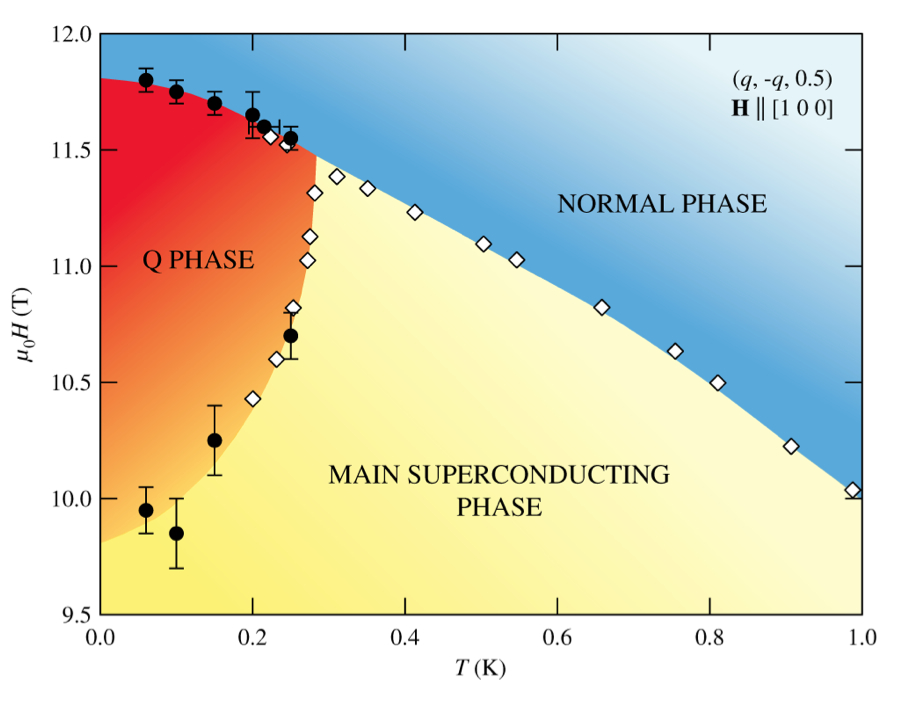
\includegraphics[width = \textwidth, height = 0.63\textwidth]{./figures/PhaseDiagramS.jpg}
					\caption{The phase diagram for CeCoIn$_5$ in the high-field low-temperature region of the $H-T$ diagram.
					\label{fig:cecoin5}}
					\end{figure}
					%%%%%%%%%%%%%%%%%%%%%%%%%%%%%%%%%%%%%%%%%%%%%%%%%%%%%%%%%%%%%%%%%%%%%
					{ \small -Kenzelmann, M. et al, Phys. Rev. Lett. 104, 127001 (2010) \\
					-Kenzelmann, M et al, Science 321, 1652 (2008) \\
					-Nicklas, M. et al, Phys. Rev. B 76, 052401 (2007) \\
					-R. Movshovich et al, in \emph{Electron Transport in Nanosystems}, pp. 127-138 (2009)}
				\end{column}
			\end{columns}
		\end{block}
		\begin{block}{\centering\veryHuge Model}
			\begin{itemize}
			\item{Superconducting 2D electrons interacting with magnetic field by Zeeman interaction}
			\item{Normal state dispersion: $\xi_{\vk}=\frac{\vk^2}{2m^*}-\epsilon_f$}
			\item{Uniform field + Perturbation: $\vH(\vR) = \vH_0 + \delta \vH_\vq e^{i\vq \cdot \vR}$}	
			\end{itemize}
			\begin{framed}		
				\bea
				\cH = \sum_{\vk,\mu} \xi_\vk c_{\vk,\mu}^\dag c_{\vk,\mu}\nonumber  + \sum_\vk \left( \Delta_\vk c_{\vk,\uparrow}^\dag c_{-\vk,\downarrow}^\dag + h.c. \right)\nonumber \\+ \mu_B\sum_{\vk,\mu,\nu} c_{\vk_+\vq,\mu}^\dag  \vsigma_{\mu\nu} (\vH_0 \delta_{\vq,0} + \delta\vH_\vq) c_{\vk,\nu}  
				\nonumber 
				\eea
			\end{framed}
				\begin{columns}[t]
				\begin{column}{0.47\linewidth}
					%%%%%%%%%%%%%%%%%%%%%%%%%%%%%%%%%%%%%%%%%%%%%%%%%%%%%%%%%%%%%%%%%%%%%
					\begin{framed}
					\begin{figure}
					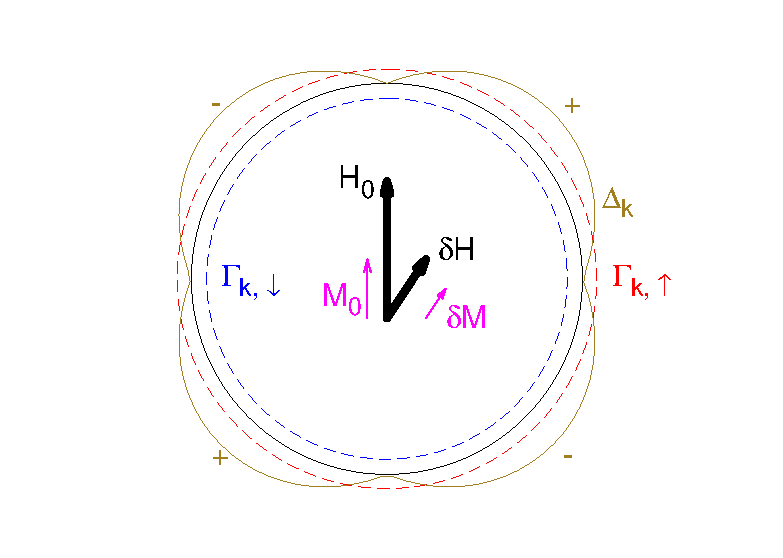
\includegraphics[scale = 1.2]{./figures/fermi_schematic.eps}
					\end{figure}
					Zeeman interaction splits Fermi surfaces for up and down spins ($\Gamma_{\vk \uparrow}, \Gamma_{\vk \downarrow}$). 
					The order parameter $\Delta_\vk \propto \sin 2\theta_\vk $ has $d$-wave symmetry. 
					\end{framed}
					%%%%%%%%%%%%%%%%%%%%%%%%%%%%%%%%%%%%%%%%%%%%%%%%%%%%%%%%%%%%%%%%%%%%%
				\end{column}
				\begin{column}{0.51\textwidth}
					\begin{center}{\LARGE Bogoliubov Transformation}\end{center}
					\begin{itemize}
					\item{New quasiparticles diagnolaize hamiltonian}
					\end{itemize}
					\begin{framed}
					{\LARGE $\Rightarrow$$\cH_0 = \sum\limits_{\vk \mu} \epsilon_{\vk \mu} \gamma^\dag_{\vk \mu} \gamma_{\vk \mu} $}
					\end{framed}
					{\small
					\bea
					c_{\vk \mu} = u_\vk \gamma_{\vk \mu} + (i\sigma_2)_{\mu\mu'} v_\vk^* \gamma^\dag_{-\vk \mu'}\\
					\epsilon_{\vk,\mu}=\sqrt{\Delta_{\vk}^2+\xi_{\vk}^2} \pm \mu_B H_0 \\
					u_{\vk}=\sqrt{\frac{1}{2}\left( 1+\frac{\xi_{\vk}}{\sqrt{\Delta_{\vk}^2+\xi_{\vk}^2}} \right)} \\
					v_{\vk}= \sgn(\Delta_\vk) \sqrt{\frac{1}{2}\left( 1-\frac{\xi_{\vk}}{\sqrt{\Delta_{\vk}^2+\xi_{\vk}^2}} \right)}
					\eea
					}
				\end{column}
			\end{columns}
		\end{block}
		
	\end{column}
	%%%%%%%%%%%%%%%%%%%%%%%%%%%%%%%%%%%%%%%%%%%%%%%%%%%%%%%%%%%%%%%%%%%%%
	%%%%%%%%%%%%%%%%%%%%%%SECOND COLUMN
	%%%%%%%%%%%%%%%%%%%%%%%%%%%%%%%%%%%%%%%%%%%%%%%%%%%%%%%%%%%%%%%%%%%%%
	\begin{column}{.59\textwidth}
		\begin{block}{\centering\veryHuge Static Antiferromagnetic Susceptibility}
			\begin{columns}[t]
				\begin{column}{0.47\textwidth}
					\bea
					M_\alpha(\vR) = M_{0\alpha}(\vH_0) + \delta M_\alpha(\vR)
					\\
					\delta M_\alpha(\vR) = \chi_{\alpha\beta} (\vq) \delta H_\beta e^{i\vq \cdot \vR}
					\eea
				\end{column}
				\begin{column}{0.47\textwidth}
					\bea
					 M_0 = \mu_B \sum\limits_{\mu} (\sigma_3)_{\mu\mu}<\psi^\dagger_{\mu}\psi_{\mu}>_{_0}
					\eea
				\end{column}
			\end{columns}
			
			\bea
			\chi_{\alpha\beta}(\vx,\vx', \omega)=-i \mu_B^2\sum\limits_{\mu\mu'\nu\nu'}\int\limits_{-\infty}^{0}dt' \; \sigma^\alpha_{\mu\mu'}\sigma^\beta_{\nu\nu'}
			e^{i\omega t'} \; 
			\langle [\psi^\dagger_\mu(\vx ',t') \psi_{\mu'}(\vx ',t'),  \psi^\dagger_\nu(\vx,0) \psi_{\nu'}(\vx,0) ]\rangle_{_0}
			\label{eq:susdef}
			\eea
			\begin{framed}
			\begin{center}{\Huge Susceptibility ($\omega=0$)}\end{center}
			\bea
			\label{eq:xi}
			\chi^{sc}_{\parallel}({\bf q})=-\mu_B^2\sum\limits_{\vk,\mu} 
			\frac{(f(\epsilon_{\vk_-\mu})-f(\epsilon_{\vk_+\mu}))(u_{\vk_+}u_{\vk_-}+v_{\vk_+}v_{\vk_-})^2}{\epsilon_{\vk_-\mu}-\epsilon_{\vk_+\mu}} 
			-\frac{(1-f(\epsilon_{\vk_-\mu})-f(\epsilon_{\vk_+\bar{\mu}}))(u_{\vk_+}v_{\vk_-}-v_{\vk_+}u_{\vk_-})^2}{\epsilon_{\vk_-\mu}+\epsilon_{\vk_+\bar{\mu}}}
			\\
			\chi^{sc}_{\perp}({\bf q})=-\mu_B^2\sum\limits_{\vk,\mu} 
			\frac{(f(\epsilon_{\vk_-\mu})-f(\epsilon_{\vk_+\bar{\mu}}))(u_{\vk_+}u_{\vk_-}+v_{\vk_+}v_{\vk_-})^2}{\epsilon_{\vk_-\mu}-\epsilon_{\vk_+\bar{\mu}}} 
			-\frac{(1-f(\epsilon_{\vk_-\mu})-f(\epsilon_{\vk_+\mu}))(u_{\vk_+}v_{\vk_-}-v_{\vk_+}u_{\vk_-})^2}{\epsilon_{\vk_-\mu}+\epsilon_{\vk_+\mu}} 
			\eea
			\end{framed}
			\begin{framed}
			\begin{columns}[t]
			\begin{column}{0.6\textwidth}
			\vspace{2cm}
				\begin{center}{ {\Huge Normal State} {\Large (Lindhard result, T = 0)}}\end{center}
				\bea
				\frac{\chi^N_\parallel(q)}{\chi^N_0}& = 1-\frac{\Theta(q-2 k_{f\uparrow})}{2}\sqrt{1-(\frac{2}{q})^2k_{f\uparrow}^2}-\frac{\Theta(q-2k_{f\downarrow})}
				{2}\sqrt{1-(\frac{2}{q})^2k_{f\downarrow}^2} \nonumber
				   \\
				\frac{\chi^N_\perp(q)}{\chi^N_0} &= 1-\Theta(q-k_{f\uparrow}-k_{f\downarrow})\sqrt{1-(\frac{2}{q})^2(1-(k_{f\uparrow}^2-k_{f\downarrow}^2)^2/(2q)^2)} 
				\nonumber
				\eea
				\begin{itemize}
				\item{$\chi_0 = 2  \mu_B^2 N_F$,\quad $\epsilon_f = 1$,\quad $k_{f\uparrow\downarrow} ^2= 1\pm \mu_B H_0/\epsilon_f$}
				\end{itemize}
			\end{column}
			\begin{column}{0.35\textwidth}
				%%%%%%%%%%%%%%%%%%%%%%%%%%%%%%%%%%%%%%%%%%%%%%%%%%%%%%%%%%%%%%%%%%%
				\begin{figure}
				 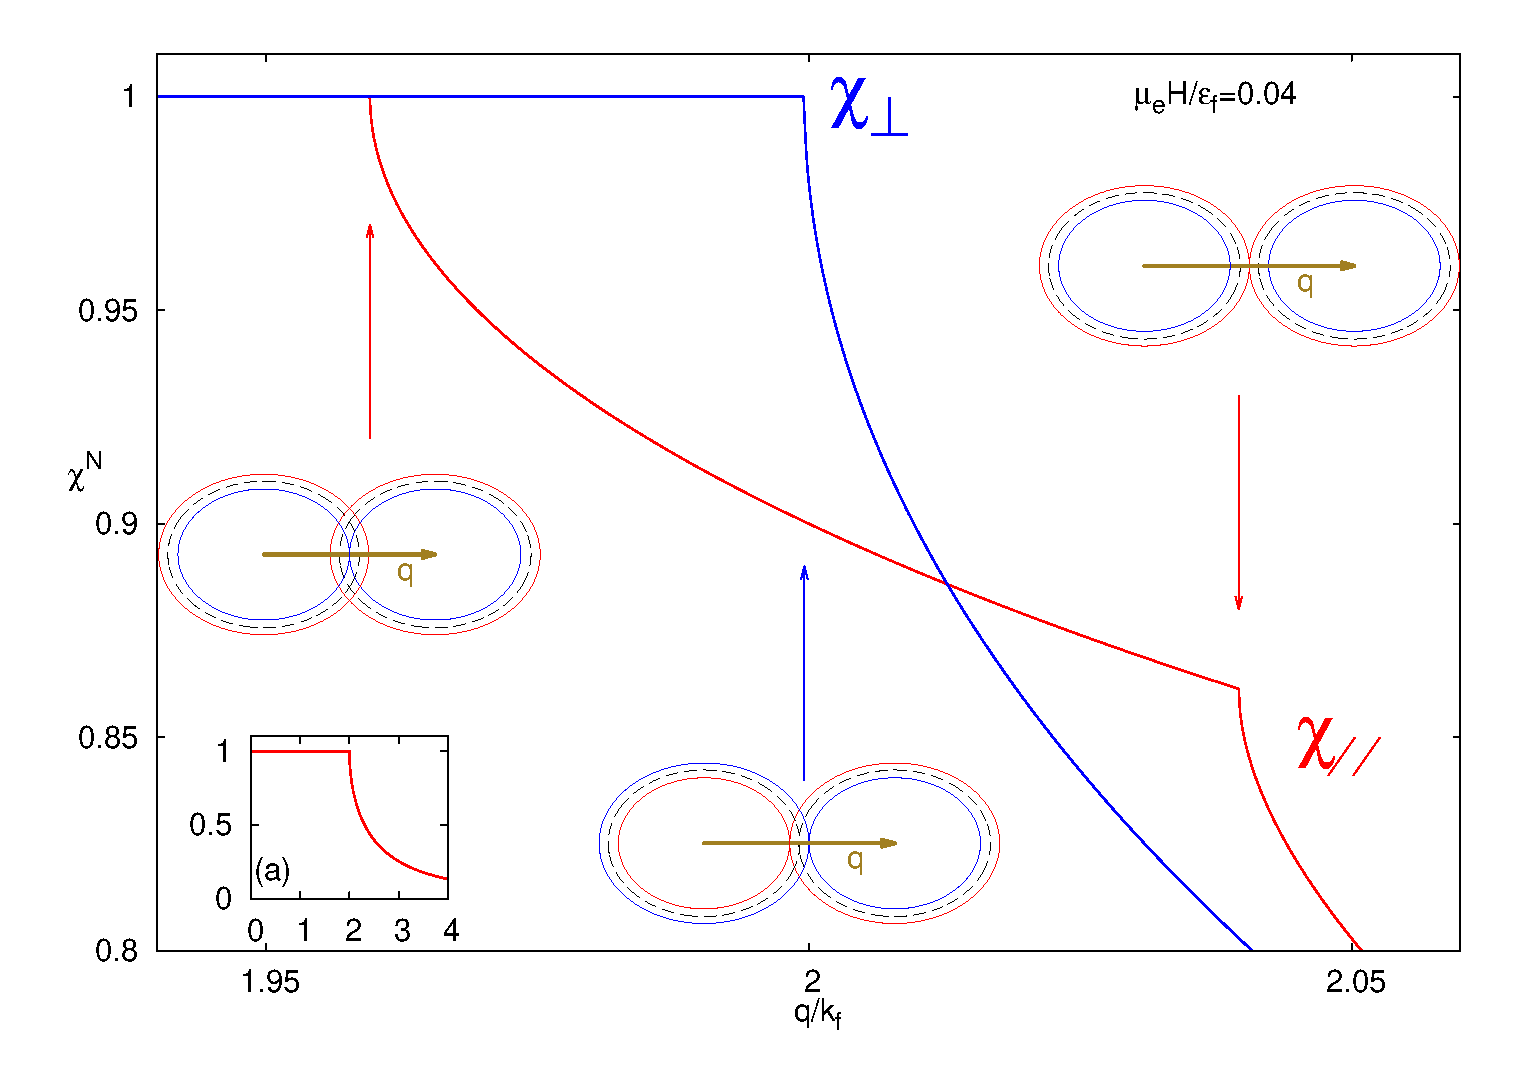
\includegraphics[height = 0.85\textwidth, width = \textwidth]{./figures/normal_chi_spin_pairing_.eps}
				 \end{figure}
				 %%%%%%%%%%%%%%%%%%%%%%%%%%%%%%%%%%%%%%%%%%%%%%%%%%%%%%%%%%%%%%%%%%%
			\end{column}
			\end{columns}
			{\bf Figure:} The 2D normal state susceptibility in zero field has a discontinuity in the first derivative at $q=2k_f$ (a). The Zeeman interaction splits this discontinuity in $\parallel$ component and leaves it intact for $\perp$
			\end{framed}


					\begin{itemize}
					\item{$\epsilon_{k\downarrow}$ gives negative quasi-particle excitations which appear as pockets near the nodes of the order 
					parameter on the new Fermi Surface (below left panel) \\
					{\small -Kato Y. et al, Phys. Rev. Lett. 107, 096401 (2011)}}
					\item{Terms in eq 9 and 10 that involve like spins give the major contributions to the enhancement of $\chi^{sc}$ (first term in $\chi_{\parallel}$ and second in $\chi_{\perp}$)}
					\item{ $\vq$'s connect opposite signs of $\Delta_\vk$ for $\chi_{\perp}$ and same signs for $\chi_{\parallel}$ (enhanced coherence factors)}
					\end{itemize}

			\begin{framed}
			\begin{columns}[t]
				\begin{column}{0.47\textwidth}
					%%%%%%%%%%%%%%%%%%%%%%%%%%%%%%%%%%%%%%%%%%%%%%%%%%%%%%%%%%%%%%%%%%%%%
					  \begin{figure}
					        \centering
					                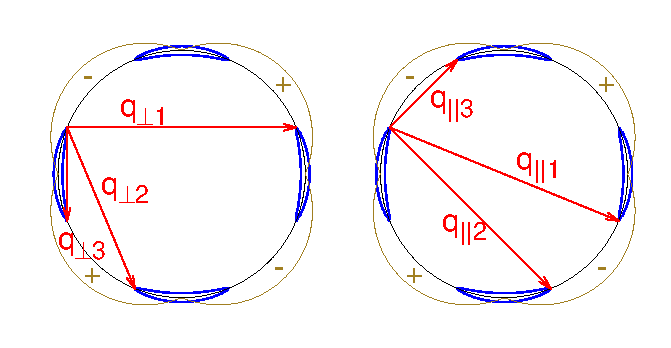
\includegraphics[width = \textwidth, height = 0.47\textwidth ]{./figures/Bananas_with_q.eps}
					 \end{figure}
					%%%%%%%%%%%%%%%%%%%%%%%%%%%%%%%%%%%%%%%%%%%%%%%%%%%%%%%%%%%%%%%%%%%%%%
					The critical wave vectors which connect points on the Fermi surface that have zero quasi-particle excitations for transverse 
					        and longitudinal AFM. The blue outlines the region inside which $\epsilon_{\vk,\downarrow}<0$, while the olive is a schematic of the order 
					        parameter
				\end{column}
				\hspace{1pt}
				\vrule
				\hspace{1pt}
				\begin{column}{0.47\textwidth}
					%%%%%%%%%%%%%%%%%%%%%%%%%%%%%%%%%%%%%%%%%%%%%%%%%%%%%%%%%%%%%%%%%%%
					 \begin{figure}
					        \centering
					                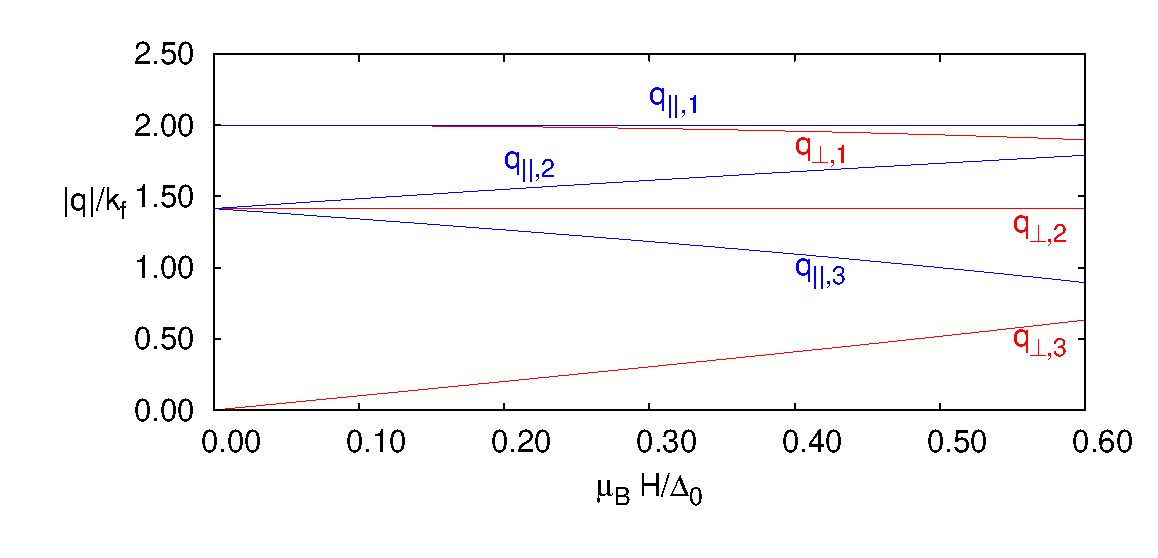
\includegraphics[width = \textwidth, height = 0.58\textwidth]{./figures/qq_theory.eps}
					
					 \end{figure}
					 Dependence of  critical $\vq$s on magnetic field
					 %%%%%%%%%%%%%%%%%%%%%%%%%%%%%%%%%%%%%%%%%%%%%%%%%%%%%%%%%%%%%%%%%%%%
				\end{column}
			\end{columns}
			\end{framed}
		\end{block}
	\end{column}
    \end{columns}
    	%%%%%%%%%%%%%%%%%%%%%%%%%%%%%%%%%%%%%%%%%%%%%%%%%%%%%%%%%%%%%%%%%%%%%
	%%%%%%%%%%%%%%%%%%%%BOTTOM PANE
	%%%%%%%%%%%%%%%%%%%%%%%%%%%%%%%%%%%%%%%%%%%%%%%%%%%%%%%%%%%%%%%%%%%%%
    \begin{block}{\centering\veryHuge Results} 			  \begin{columns}[t]
			  	
			  	\begin{column}{0.5\textwidth}
			 	\begin{column}{0.6\textwidth}
					\vspace{-2cm}
					 %%%%%%%%%%%%%%%%%%%%%%%%%%%%%%%%%%%%%%%%%%%%%%%%%%%%%%%%%%%%%%%%%%%%
					 \begin{figure}
					 \label{fig:xx_enh}
					        \centering
					                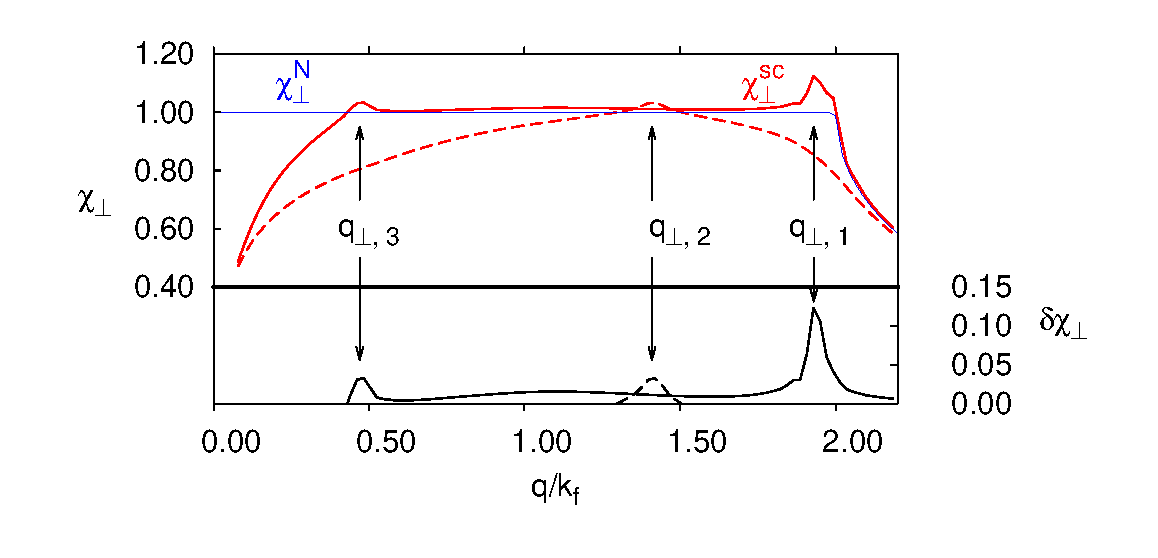
\includegraphics[scale = 1.4]{./figures/enhanced_chi_xx.eps}
					 \end{figure}
					 %%%%%%%%%%%%%%%%%%%%%%%%%%%%%%%%%%%%%%%%%%%%%%%%%%%%%%%%%%%%%%%%%%%%%%
					\vspace{-2cm}
					%%%%%%%%%%%%%%%%%%%%%%%%%%%%%%%%%%%%%%%%%%%%%%%%%%%%%%%%%%%%%%%%%%%%%
					 \begin{figure}
					 \label{fig:zz_enh}
					        \centering
					                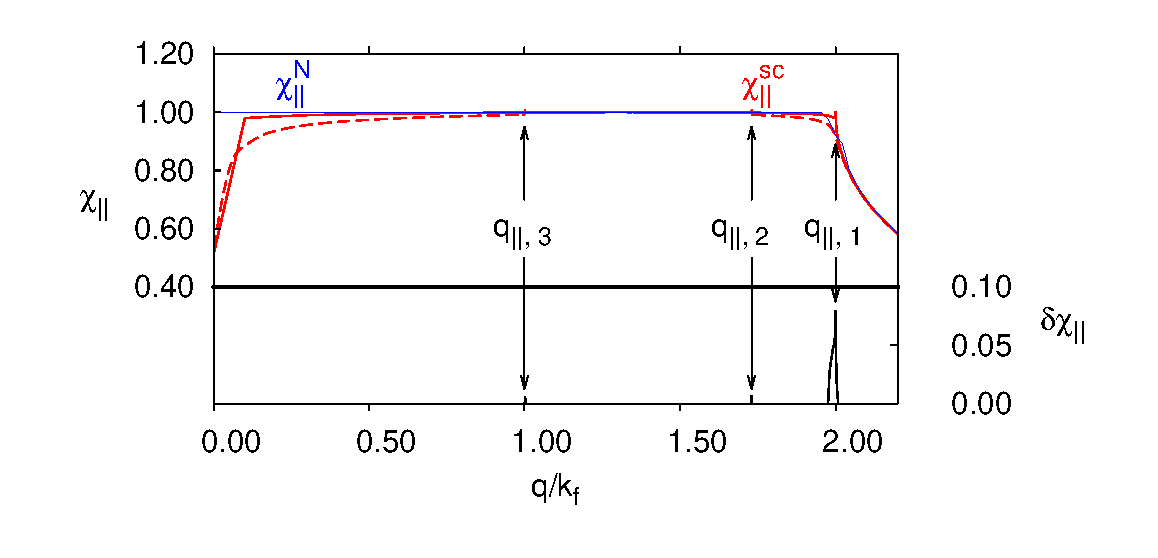
\includegraphics[scale = 1.4]{./figures/enhanced_chi_zz.eps}
					    \end{figure}
					 %%%%%%%%%%%%%%%%%%%%%%%%%%%%%%%%%%%%%%%%%%%%%%%%%%%%%%%%%%%%%%%%%%%%%
				\end{column}
				\begin{column}{0.35\textwidth}
					\vspace{3cm}\\
			  		The upper panes show the normlaized susceptibility in the superconducting state (red) as a function of q, which shows
					                 enhancement over the normal state (blue) at the expected wave vectors. The lower panes shows $\delta\chi_\perp(\vq) =( \chi_\perp^{sc}(\vq) - \chi_\perp^{N}(\vq))/\chi_0$.   $\mu_B H = 0.5\Delta_0,\quad T=0$ \\
				{\bf Top:} The solid red line is along the nodal direction, while the dotted line is taken along the direction of $\vq_{\perp 2}$. $\Delta_0 = 0.1\epsilon_f$\\
				{\bf Bottom:} The solid red line is along the $\vq_{\parallel,1}$ direction, while the dotted line is taken along the direction of $\vq_{\parallel 2}$. $\Delta_0 = 0.01\epsilon_f$
				\end{column}
				\end{column}
				
				\vrule{}
				
				\begin{column}{0.3\textwidth}\\
				\vspace{1cm}
				\begin{itemize}
				\item{
				If denominator of total susceptibility is close to zero, a small enhancement of $\chi$ may be enough to cause ordered state.
				}
				\end{itemize}
				\begin{center}
				 \fbox{{\huge${\bf \chi}^{tot}_{\alpha\beta}(\vq) = \frac{\chi_{\alpha\beta}(\vq)}{1-J_{\alpha\beta}(\vq)\chi_{\alpha\beta}(\vq)}$}}
				 \end{center}
				%%%%%%%%%%%%%%%%%%%%%%%%%%%%%%%%%%%%%%%%%%%%%%%%%%%%%%%%%%%%%%%%%%%%%%
				 \begin{figure}
				

				 \label{fig:xx_cont}
				        \centering
				                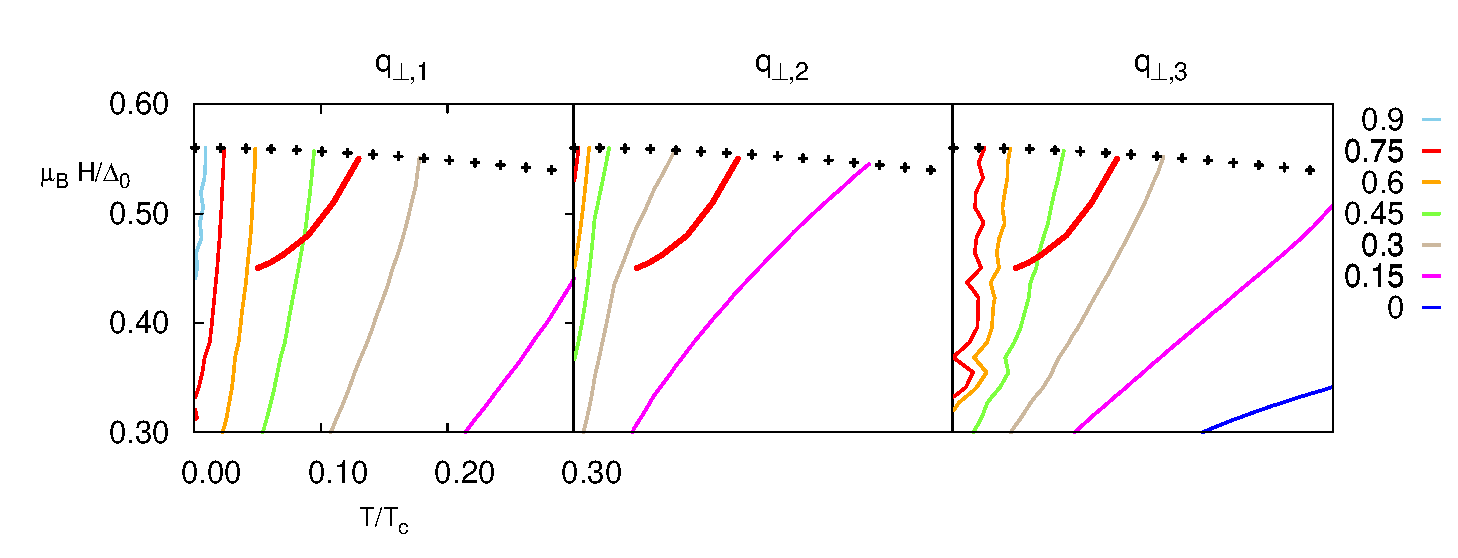
\includegraphics[scale = 1]{./figures/xx_all_enhanced_q.eps}
				 \end{figure}
				 %%%%%%%%%%%%%%%%%%%%%%%%%%%%%%%%%%%%%%%%%%%%%%%%%%%%%%%%%%%%%%%%%%%%%%%%
				Percent increase of $\chi_{\perp}$ for the critical wave vectors, $(\delta\chi_{\perp}(\vq) \%)$. The black crosses outline the first 
				                order phase transition for a Pauli limited d-wave superconductor, and the bold red line is a qualitative sketch of the Q-phase boundary of 
				                CeCoIn$_5$. $\Delta_0 = 0.005\epsilon_f$
			 \end{column}
			 \vrule{}
			 \begin{column}{0.18\textwidth}
			  		%%%%%%%%%%%%%%%%%%%%%%%%%%%%%%%%%%%%%%%%%%%%%%%%%%%%%%%%%%%%%%%%%%
					 \begin{figure}
					        \centering
					                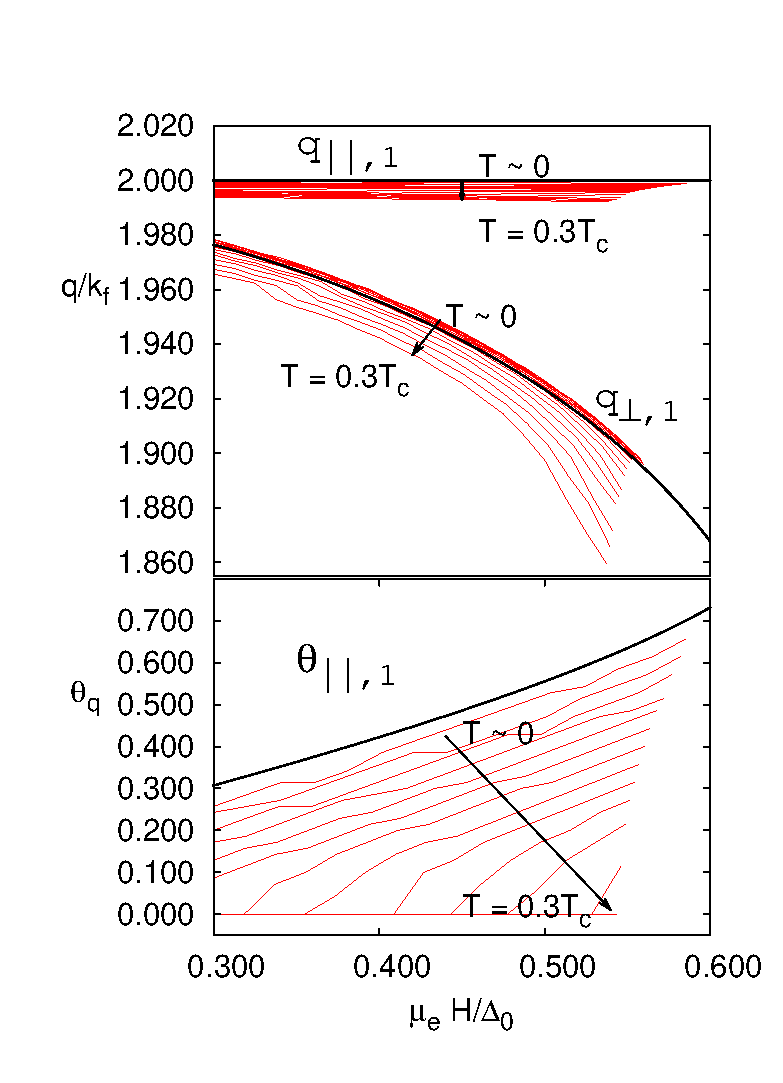
\includegraphics[width = 1\textwidth, height = 1\textwidth]{./figures/max_q_T.eps}
					 \end{figure}
					 %%%%%%%%%%%%%%%%%%%%%%%%%%%%%%%%%%%%%%%%%%%%%%%%%%%%%%%%%%%%%%%%%%%
					 The numerically found $\vq$ for which $\delta\chi$ is maximized (red). The black
					                 lines are the theoretical curves for $\vq_{\parallel,1}$ and $\vq_{\perp,1}$. \\$\Delta_0 = 0.005\epsilon_f$
				\end{column}
			\end{columns}
 
		\end{block}
  \end{frame}
  \end{document}
